\chapter{OSDOCR Pipeline - Implementação}
\label{cap_osdocr_pipeline_implementacao}

Neste capítulo, será explorada a implementação da componente de pipeline.

De forma a criar um caso de uso para as ferramentas criadas e outras exploradas e disponibilizadas, foi criado um comando de aplicação de uma pipeline de aplicação de OCR, que permite, a partir de uma imagem: aplicar tratamentos para melhorar a sua qualidade; aplicar OCR; tratar os resultados; e gerar um output simples, ou específico para jornais.

Através dos argumentos passados à ferramenta, a pipeline consegue comportar-se de forma diferente, por exemplo: aceitar como output inicial uma instância de Hocr ou de OCR Tree em formato JSON; ignorar pré-processamento ou passos específicos deste; etc.

As funcionalidades disponíveis na pipeline são uma culminação do trabalho descrito anteriormente sobre o OSDOCR Toolkit, assim como ferramentas exploradas para resolver questões que este não aborda como, por exemplo, realização de upscaling de uma imagem.

Como discutido no estudo da solução, os blocos que compõem a pipeline são, sempre que possível, opcionais de modo a aumentar a sua versatilidade.

Além disso, dependendo do modo de utilização da pipeline, output extra pode ser requisitado. Utilizando a flag de debug ('-d' ou '--debug') cada um dos blocos da pipeline irá guardar o seu resultado na forma de um ficheiro situado na diretoria de resultados do input respetivo. 

\section{Sumário}

O comando de invocação da pipeline é 'osdocr'. Este apresenta as seguintes opções de utilização:

\begin{itemize}\setlength\itemsep{-0.8em}
	\item \textbf{target} 
		\begin{itemize}\setlength\itemsep{-0.5em}
			\item \textbf{alternativo} : t
			\item \textbf{descrição} : ficheiro de imagem a ser processado pela pipeline.
		\end{itemize}
		
	\item \textbf{file}
		\begin{itemize}\setlength\itemsep{-0.5em}
			\item \textbf{alternativo} : f
			\item \textbf{descrição} : ficheiro de texto que lista um target por linha.
		\end{itemize}
		
	\item \textbf{target\_ocr\_results} 
		\begin{itemize}\setlength\itemsep{-0.5em}
			\item \textbf{alternativo} : tocr
			\item \textbf{descrição} : ficheiro de resultados OCR. Pode ser de tipo hocr ou json. Se fornecido, não será realizado pré processamento de imagem ou OCR.
		\end{itemize}
		
	\item \textbf{output\_folder}
		\begin{itemize}\setlength\itemsep{-0.5em}
			\item \textbf{alternativo} : of
			\item \textbf{descrição} : caminho para guardar os resultados
		\end{itemize}
		
	
	\item \textbf{segmented\_ocr}
		\begin{itemize}\setlength\itemsep{-0.5em}
			\item \textbf{alternativo} : sgocr
			\item \textbf{descrição} : flag para aplicação de OCR no target será realizada em cada um dos segmentos, invés de na imagem inteira. Cada uma das partes é posteriormente unida para criar uma única OCR Tree de resultados.
			\item \textbf{valor default} : False
		\end{itemize}
		
	\item \textbf{target\_segments}
		\begin{itemize}\setlength\itemsep{-0.5em}
			\item \textbf{alternativo} : ts
			\item \textbf{descrição} : segmentos a calcular no target. Segmento body é sempre obtido. O body é ainda repartido nas suas colunas.
			\item \textbf{opções} : 'header', 'body', 'footer'
			\item \textbf{valor default} : 'header','body'
		\end{itemize}
		
	\item \textbf{force\_ocr}
		\begin{itemize}\setlength\itemsep{-0.5em}
			\item \textbf{alternativo} : focr
			\item \textbf{descrição} : flag que ignora possíveis ficheiros em cache de resultados OCR, consequentes de iterações anteriores do target. Força aplicação de na imagem.
			\item \textbf{valor default} : False
		\end{itemize}
		
	\item \textbf{tesseract\_config}
		\begin{itemize}\setlength\itemsep{-0.5em}
			\item \textbf{descrição} : flags para serem passadas ao Tesseract no momento de aplicação de OCR. Estas estão disponíveis na documentação do Tesseract. Cada argumento tem de ter como prefixo '\_\_' para permitir o seu processamento.
			\item \textbf{valor default} : \_\_l por
		\end{itemize}
	
	\item \textbf{text\_confidence}
		\begin{itemize}\setlength\itemsep{-0.5em}
			\item \textbf{alternativo} : tc
			\item \textbf{descrição} : valor de confiança de texto que pipeline irá usar.
			\item \textbf{valor default} : 10
		\end{itemize}
	
	
	\item \textbf{split\_whitespace}
		\begin{itemize}\setlength\itemsep{-0.5em}
			\item \textbf{alternativo} : sw
			\item \textbf{descrição} : valor utilizado como razão entre um espaço branco num bloco de texto e a média pesada dos espaçamentos entre palavras, para este ser considerado válido como ponto de divisão de um bloco.
			\item \textbf{valor default} : 3
		\end{itemize}
	
	\item \textbf{fix\_rotation}
		\begin{itemize}\setlength\itemsep{-0.5em}
			\item \textbf{alternativo} : fr
			\item \textbf{descrição} : opções usadas para a correção de rotação de documento.
			\item \textbf{opções} : 'auto','clockwise','counter-clockwise'
			\item \textbf{valor default} : 'auto'
		\end{itemize}
	
	\item \textbf{upscaling\_image}
		\begin{itemize}\setlength\itemsep{-0.5em}
			\item \textbf{alternativo} : upi
			\item \textbf{descrição} : opções usadas para o upscaling de imagem. Se opção 'autoscale' do modelo 'waifu2x' for escolhido, aplica upscaling da imagem até esta chegar ao dpi alvo (opção target\_dpi).
			\item \textbf{opções} : 'waifu2x' -> 'scale2x', 'scale4x', 'autoscale'
			\item \textbf{valor default} : 'waifu2x'
		\end{itemize}
	
	\item \textbf{target\_dpi}
		\begin{itemize}\setlength\itemsep{-0.5em}
			\item \textbf{alternativo} : tdpi
			\item \textbf{descrição} : valor do dpi alvo
			\item \textbf{valor default} : 300
		\end{itemize}
	
	\item \textbf{target\_dimensions}
		\begin{itemize}\setlength\itemsep{-0.5em}
			\item \textbf{alternativo} : tdim
			\item \textbf{descrição} : valor das dimensões físicas a usar para cálculo do dpi da imagem. Opções estão disponíveis no ficheiro 'dimensions.json' no projeto, podendo ser atualizado.
			\item \textbf{opções} : 'A5', 'A4', 'A3', 'A2', 'A1', 'A0', '2A0'
			\item \textbf{valor default} : A3
		\end{itemize}
	
	\item \textbf{denoise\_image}
		\begin{itemize}\setlength\itemsep{-0.5em}
			\item \textbf{alternativo} : di
			\item \textbf{descrição} : opções usadas para o denoising de imagem.
			\item \textbf{opções} : 'waifu2x' -> '-1' - '3'
			\item \textbf{valor default} : 'waifu2x'
		\end{itemize}
	
	\item \textbf{light\_correction}
		\begin{itemize}\setlength\itemsep{-0.5em}
			\item \textbf{alternativo} : lc
			\item \textbf{descrição} : opções usadas para a correção de iluminação de uma imagem.
			\item \textbf{opções} : 'best\_SSIM', 'best\_PSNR', 'LOL-Blur', 'SICE', 'SID', 'w\_perc'
			\item \textbf{valor default} : 'best\_SSIM'
		\end{itemize}
		
	\item \textbf{light\_correction\_split\_image}
	\begin{itemize}\setlength\itemsep{-0.5em}
		\item \textbf{alternativo} : lcs
		\item \textbf{descrição} : flag para aplicação de correção de iluminação da imagem em patches, invés de na totalidade, de modo a melhorar tempo de processamento. Para certos modelos, resulta em contrastes consideráveis entre os patches.
		\item \textbf{valor default} : True
	\end{itemize}
	
	\item \textbf{binarize\_image}
		\begin{itemize}\setlength\itemsep{-0.5em}
			\item \textbf{alternativo} : bi
			\item \textbf{descrição} : opções usadas para a binarização de imagem para aplicação de OCR.
			\item \textbf{opções} : 'fax', 'otsu'
			\item \textbf{valor default} : 'fax'
		\end{itemize}
	
	\item \textbf{remove\_document\_images}
		\begin{itemize}\setlength\itemsep{-0.5em}
			\item \textbf{alternativo} : bi
			\item \textbf{descrição} : método utilizado para remoção de imagens.
			\item \textbf{opções} : 'leptonica', 'layoutparser'
			\item \textbf{valor default} : 'leptonica'
		\end{itemize}
	
	\item \textbf{target\_old\_document}
		\begin{itemize}\setlength\itemsep{-0.5em}
			\item \textbf{alternativo} : tod
			\item \textbf{descrição} : flag para indicar que target é um documento antigo. Utilizado quando método 'layoutparser' é escolhido, de forma a escolher o modelo mais apropriado
			\item \textbf{valor default} : True
		\end{itemize}
	
	\item \textbf{ignore\_delimiters}
		\begin{itemize}\setlength\itemsep{-0.5em}
			\item \textbf{alternativo} : igd
			\item \textbf{descrição} : flag para ignorar delimitadores. Se ativada, estes não serão tidos em conta como indicadores do layout do documento no cálculo da ordem de leitura.
			\item \textbf{valor default} : False
		\end{itemize}
	
	\item \textbf{skip\_method}
		\begin{itemize}\setlength\itemsep{-0.5em}
			\item \textbf{descrição} : métodos/passos da pipeline a ignorar.
			\item \textbf{opções} : 'leptonica', 'layoutparser'
			\item \textbf{valor default} : 'all', 'auto\_rotate', 'noise\_removal', 'blur\_removal', 'light\_correction', 'image\_preprocess', 'remove\_document\_margins', 'remove\_document\_images', 'image\_upscaling', 'identify\_document\_delimiters', 'binarize\_image', 'clean\_ocr', 'split\_whitespace', 'unite\_blocks', 'calculate\_reading\_order', 'extract\_articles', 'posprocessing'
		\end{itemize}
	
	\item \textbf{calibrate}
		\begin{itemize}\setlength\itemsep{-0.5em}
			\item \textbf{descrição} : aplicar modo de calibração de pipeline. Usado para encontrar melhor configuração de pipeline para um dado target. Pode ser dado um diretório onde estarão disponíveis os ficheiros necessários para calibração, e onde ficarão os resultados de calibração; e um diretório com configurações de pipeline a testar. Por defeito, o diretório procurado dá-se por 'calibration' no local onde o comando foi corrido, e são usadas configurações de pipeline disponíveis no projeto. 
		\end{itemize}
	
	\item \textbf{calibrate\_no\_reuse}
		\begin{itemize}\setlength\itemsep{-0.5em}
			\item \textbf{descrição} : flag para não utilizar cache existente.
			\item \textbf{valor default} : False
		\end{itemize}
	
	\item \textbf{pipeline\_config}
		\begin{itemize}\setlength\itemsep{-0.5em}
			\item \textbf{descrição} : ficheiro do tipo JSON com configuração de pipeline a usar. Pode ser usado como alternativa a aplicar argumentos no terminal de comandos.
		\end{itemize}
		
	\item \textbf{gui}
		\begin{itemize}\setlength\itemsep{-0.5em}
			\item \textbf{descrição} : aplicar modo de interface gráfica. Interface gráfica simples que pode ser utilizada para experimentar algumas das funcionalidades disponíveis. Maioritariamente usada para debugging.
		\end{itemize}
\end{itemize}


\section{Pré-processamento de imagem}

Como primeiro procedimento da pipeline, no caso de uso de inputs de imagem, tem-se o tratamento desta, para procurar obter, a partir da aplicação OCR, uma melhor transcrição do conteúdo textual, assim como melhor identificação de outros elementos, como figuras.

Para isso, procurou-se abordar os seguintes problemas: imagens rodadas; remoção de margens/sombras na margem de documentos; imagens de baixa resolução; remoção de figuras de documentos; imagens com ruído; imagens com distribuição de iluminação inconsistente;.

As solução destes problemas envolveram o uso de métodos desenvolvidos no toolkit, assim como soluções já existentes.

A ordem de aplicação destas soluções mostrou ser relevante pois estas podem interferir umas com as outras, por exemplo: aplicação de denoising antes de remover as figuras do documento pode afetar a identificação destas. Assim sendo, a ordem ótima de execução segue a listagem que se segue.

\begin{figure}[H]
	\centering
	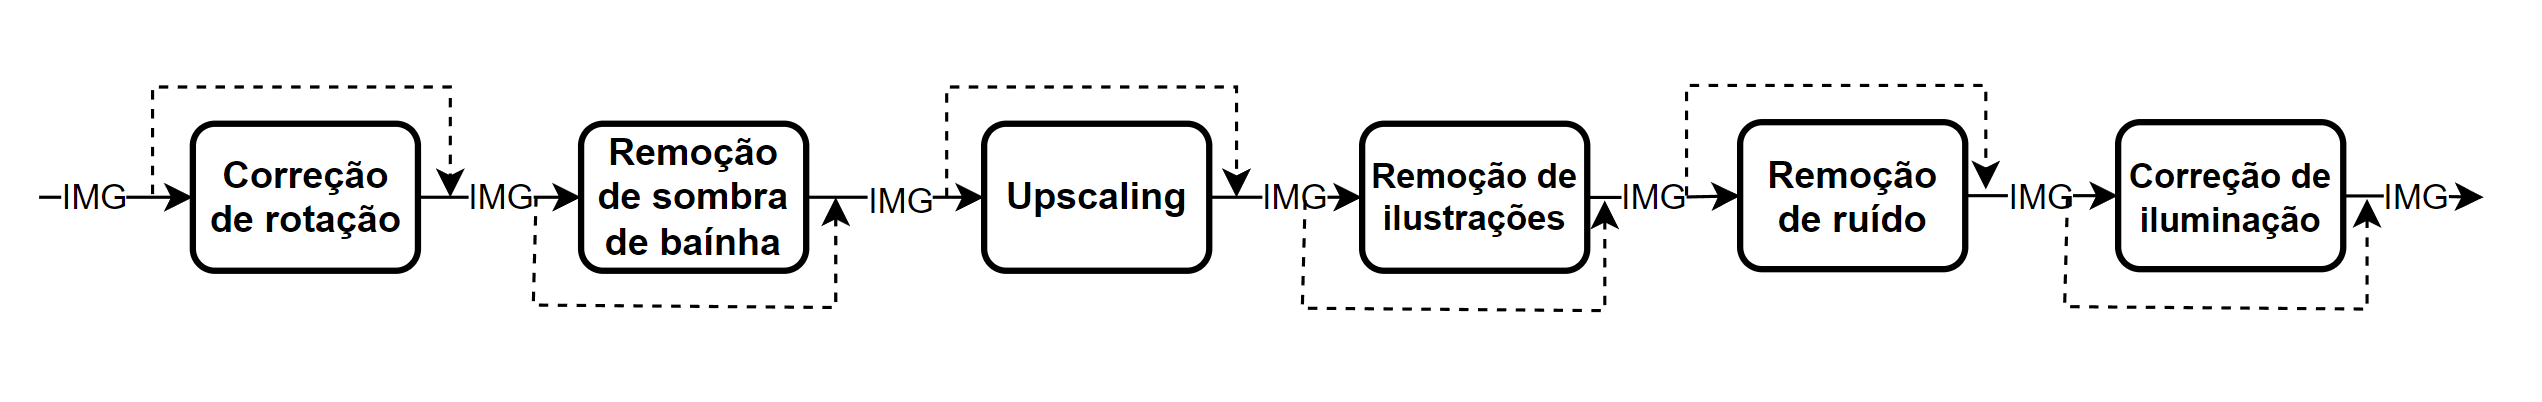
\includegraphics[width=1\textwidth]{images/diagramas/arquitetura_pipeline_preprocess.png}
	\caption{Pipeline - secção pré-processamento}
	\label{fig:arquitetura_pipeline_preprocess}
\end{figure}

\highlight{Correção de rotação}

A correção de possíveis rotações de imagens de documentos é resolvida utilizando os métodos de correção de rotação descritos na secção de métodos de processamento de imagem.

\highlight{Remoção de sombras das margens do documento}

De igual modo, a remoção de possíveis sombras na margem de um documento aproveita os métodos desenvolvidos e descritos para este efeito na mesma secção. 

A aplicação desta funcionalidade deve vir após a correção de possíveis rotações pois, como esta solução envolve a análise da distribuição dos valores de pixeis, se estas sombras se apresentarem inclinadas a possibilidade que elas não sejam resolvidas aumenta.


\highlight{Upscaling de imagem}

Para a resolução de problemas resultantes de imagens com baixos valores de dpi, modelos de Deep Learning obtém resultados mais interessantes em relação a algoritmos passados, como interpolação. Dentro destes modelos, o \href{https://github.com/nagadomi/waifu2x}{waifu2x} é bastante respeitado no que toca a aumento de resolução de imagem e limpeza de imperfeições. 

Embora não especificamente focado para o processamento de imagens de documentos, o seu fácil uso e instalação, assim como a verificação de bons resultados mesmo nesta área relativamente externa ao treino, levaram a que este modelo seja uma boa adição às ferramentas de pré-processamento de imagem disponíveis na pipeline.

Esta funcionalidade, quando escolhida para realizar upscaling automático, é dependente das configurações utilizadas para cálculo de dpi de imagem (dimensões reais proporcionadas).

A aplicação de OCR é recomendada para dpi no valor de 300 ou superior, sendo que para imagens antigas, esta funcionalidade é essencial.


\begin{figure}[H]
	\centering
	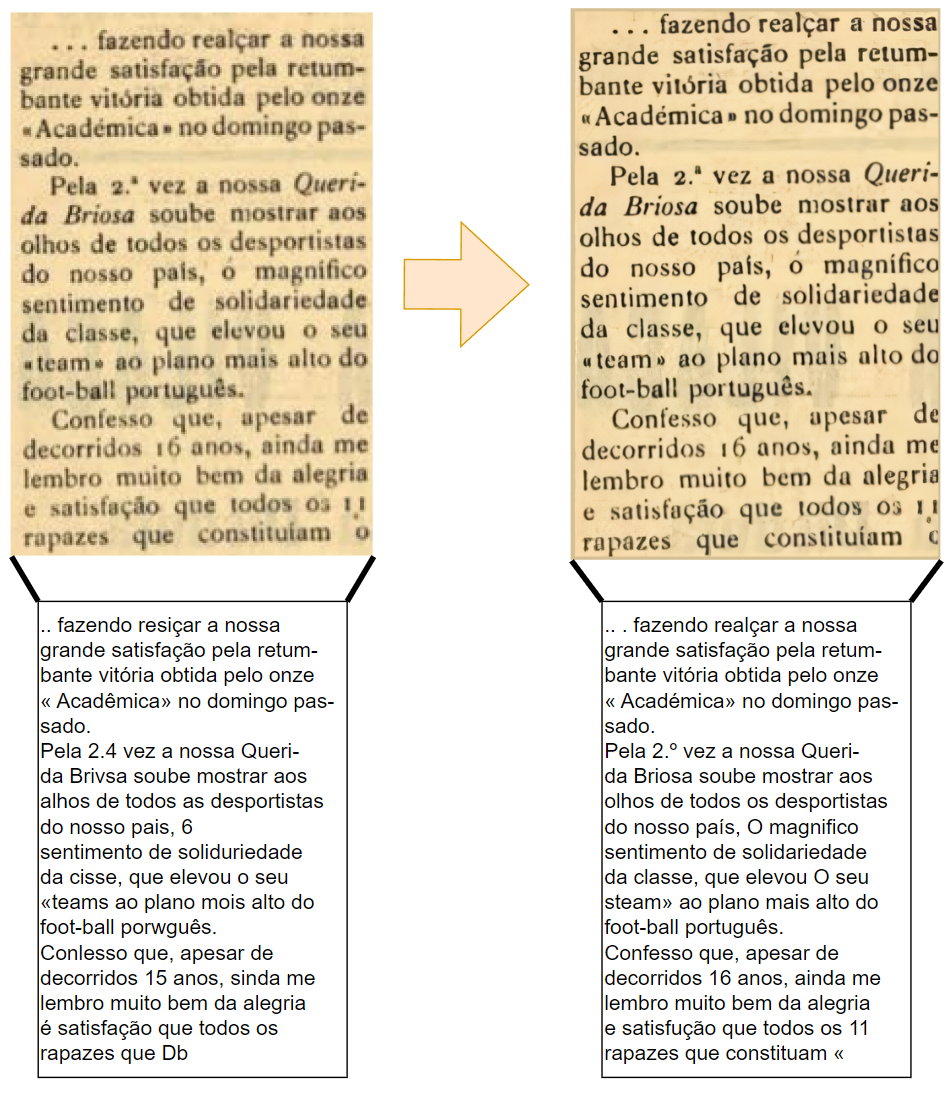
\includegraphics[width=0.7\textwidth]{images/ilustracoes/upscaling_example.png}
	\caption{Exemplo de diferença de OCR numa secção de texto sem (esquerda) e com (direita) upscaling. Upscaling realizado foi apenas de 2x, utilizando o modelo waifu2x.}
	\label{fig:upscaling_example}
\end{figure}


\highlight{Remoção de ilustrações de documento}

De forma a diminuir a presença de elementos não identificados nos resultados OCR, assim como permitir identifica-los corretamente, esta funcionalidade procura remover as ilustrações de um documento, recortando-as para uma pasta temporário, permitindo a sua reposição na imagem final.

Entre as soluções exploradas para esta questão, a que se enquadrava mais na questão de identificação de ilustrações de documentos, e até com atenção a jornais, foi o modelo \href{https://layout-parser.readthedocs.io/en/latest/index.html}{Layout Parser}, mais especificamente, aproveitando o modelo Detectron desenvolvido pela Meta.
Este, no entanto, apresenta uma instalação complexa devido a dependências de bibliotecas da própria Meta que demonstram incompatibilidades e que necessitam ser modificadas manualmente.

Deste modo, aproveitou-se uma alternativa com resultados também satisfatórios e de menor custo computacional, com métodos de segmentação de documento propostos pela Leptonica. Estes foram descritos também na secção anterior.

Comparando os dois, a opção de usar Leptonica é satisfatória na generalidade dos casos, até identificando com maior precisão as ilustrações (delimitando menos fundo do documento) em vários casos de estudo. Os métodos de Leptonica tendem no entanto a errar para ilustrações que não apresentem uma borda notável e tenham um fundo similar ao fundo do documento. Nestes casos, o Layout Parser é mais propício a acertar.

\begin{figure}[H]
	\centering
	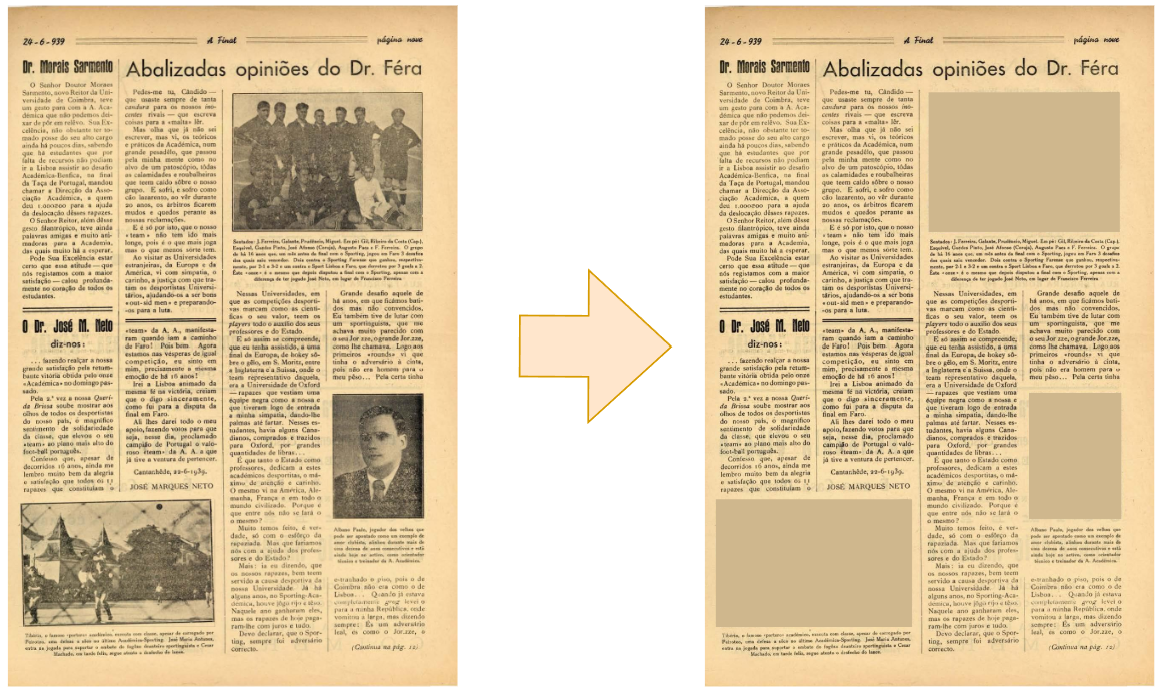
\includegraphics[width=0.6\textwidth]{images/ilustracoes/remove_images_example.png}
	\caption{Exemplo de resultado de passo de remoção das imagens identificadas.}
	\label{fig:remove_images_example}
\end{figure}



É também importante realçar que a pipeline, no processo de recortar as ilustrações, preenche o espaço vazio com uma média das cores de fundo da imagem. Este passo é importante pois caso contrário a binarização posterior da imagem, dependendo da distribuição das cores desta, pode resultar numa imagem inutilizável.

\begin{figure}[H]
	\centering
	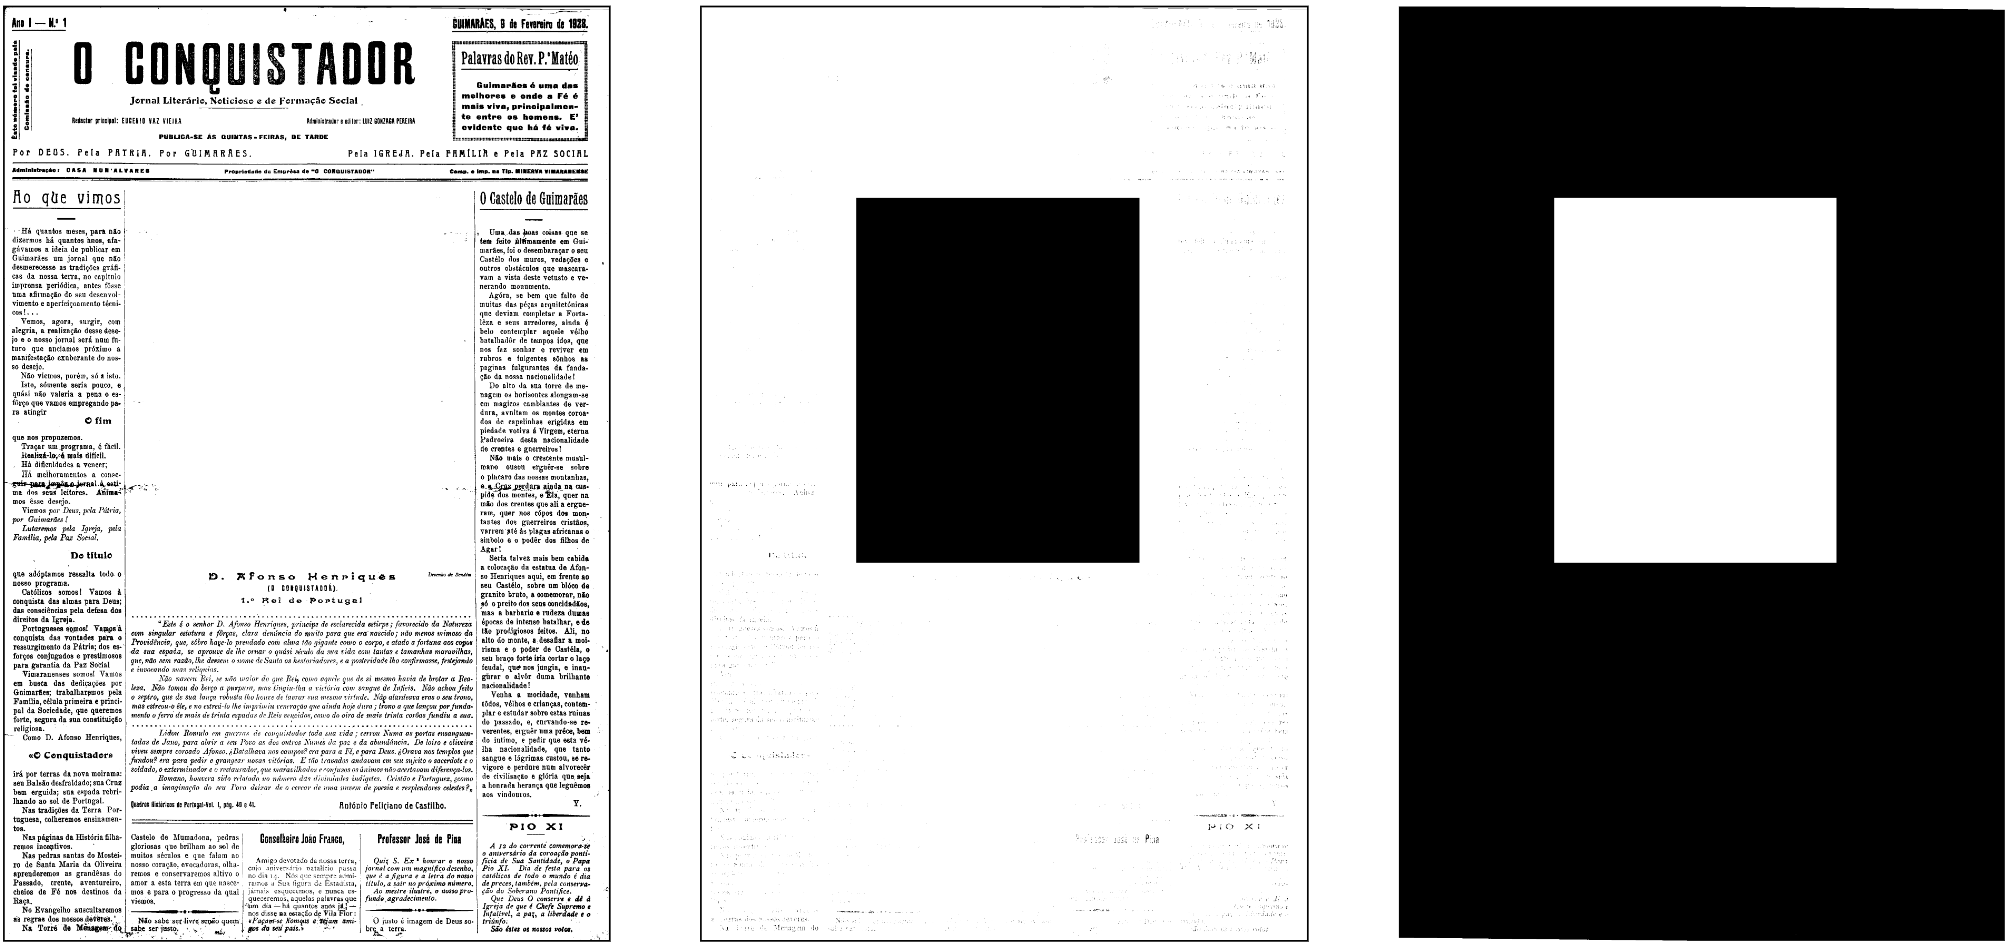
\includegraphics[width=0.7\textwidth]{images/ilustracoes/binarize_remove_images_example.png}
	\caption{Resultado de binarização correspondente a diferentes preenchimentos da zona das ilustrações removidas. Esquerda: preenchido com a cor média da imagem; Meio: preenchido com branco; Direita: preenchido com preto.}
	\label{fig:binarize_remove_images_example}
\end{figure}

\highlight{Denoising de imagem}

Para a realização de denoising, foi também aplicado o modelo de \textbf{waifu2x}, visto este proporcionar opções para este efeito. Este denoising é realizado em imagens a cor, sendo portanto subtil.

O denoising mais relevante é realizado na binarização realizada antes da aplicação de OCR.

\begin{figure}[H]
	\centering
	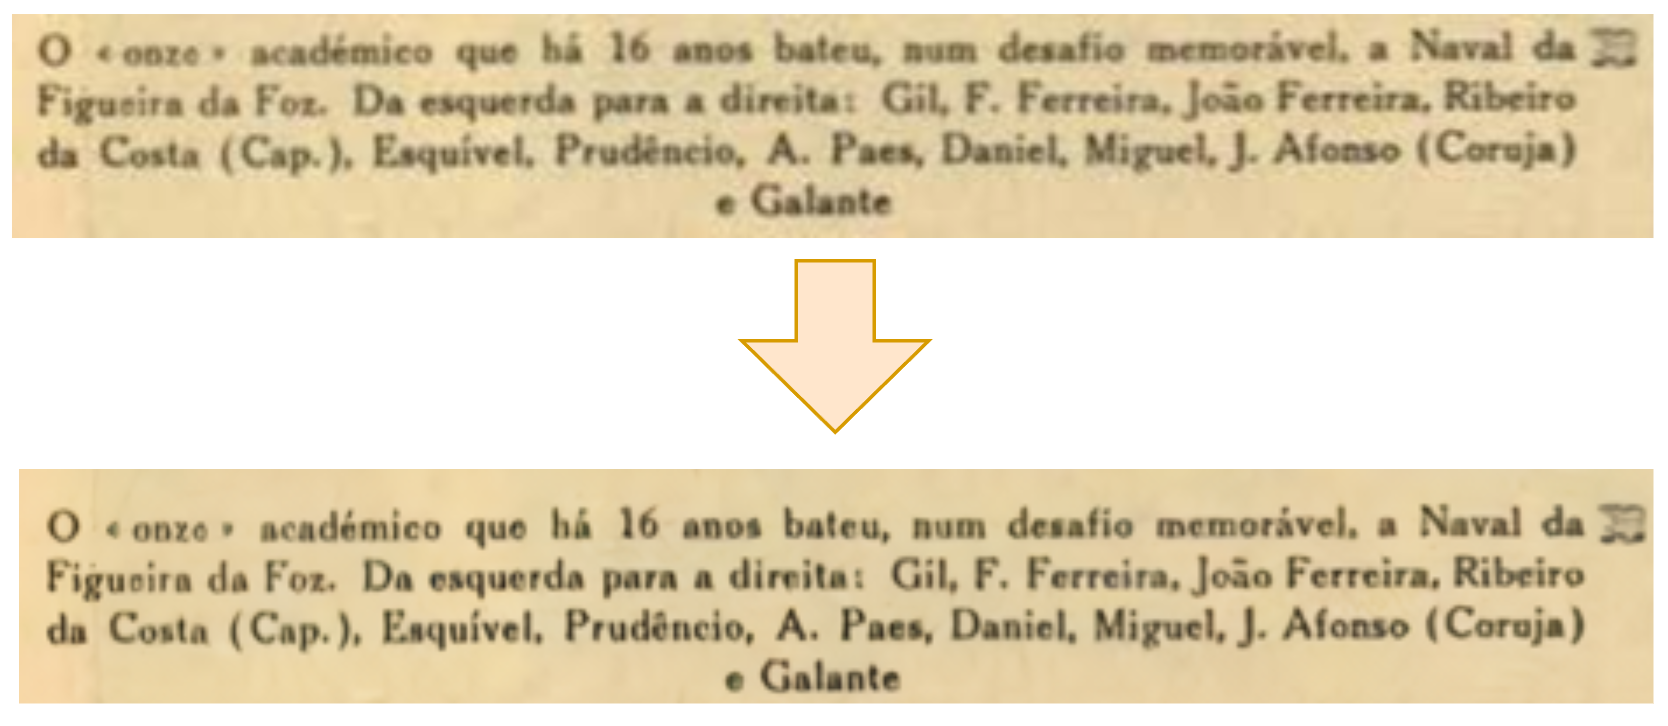
\includegraphics[width=0.7\textwidth]{images/ilustracoes/denoise_example.png}
	\caption{Resultado de modelo de denoise do waifu2x.}
	\label{fig:denoise_example}
\end{figure}



\highlight{Correção de iluminação}

Para a correção de iluminação de documentos, também se conclui que modelos de Deep Learning são a melhor opção. A família de modelos que mostraram resultados mais interessantes e com instalação simples foi \href{https://github.com/Fediory/HVI-CIDNet}{HVI-CIDNet}. Os pesos para estes estão disponibilizados nesse mesmo repositório.

Para imagens de maior resolução, o tempo de processamento destes modelos é considerável, sendo que como solução a pipeline apresenta uma opção para dividir a imagem em patches e correr o modelo em cada um destes, unindo-os no final. Para alguns modelos, esta divisão pode resultar em contrastes notáveis na imagem, particularmente para imagens de maior resolução (por ser repartido em mais patches).

\begin{figure}[H]
	\centering
	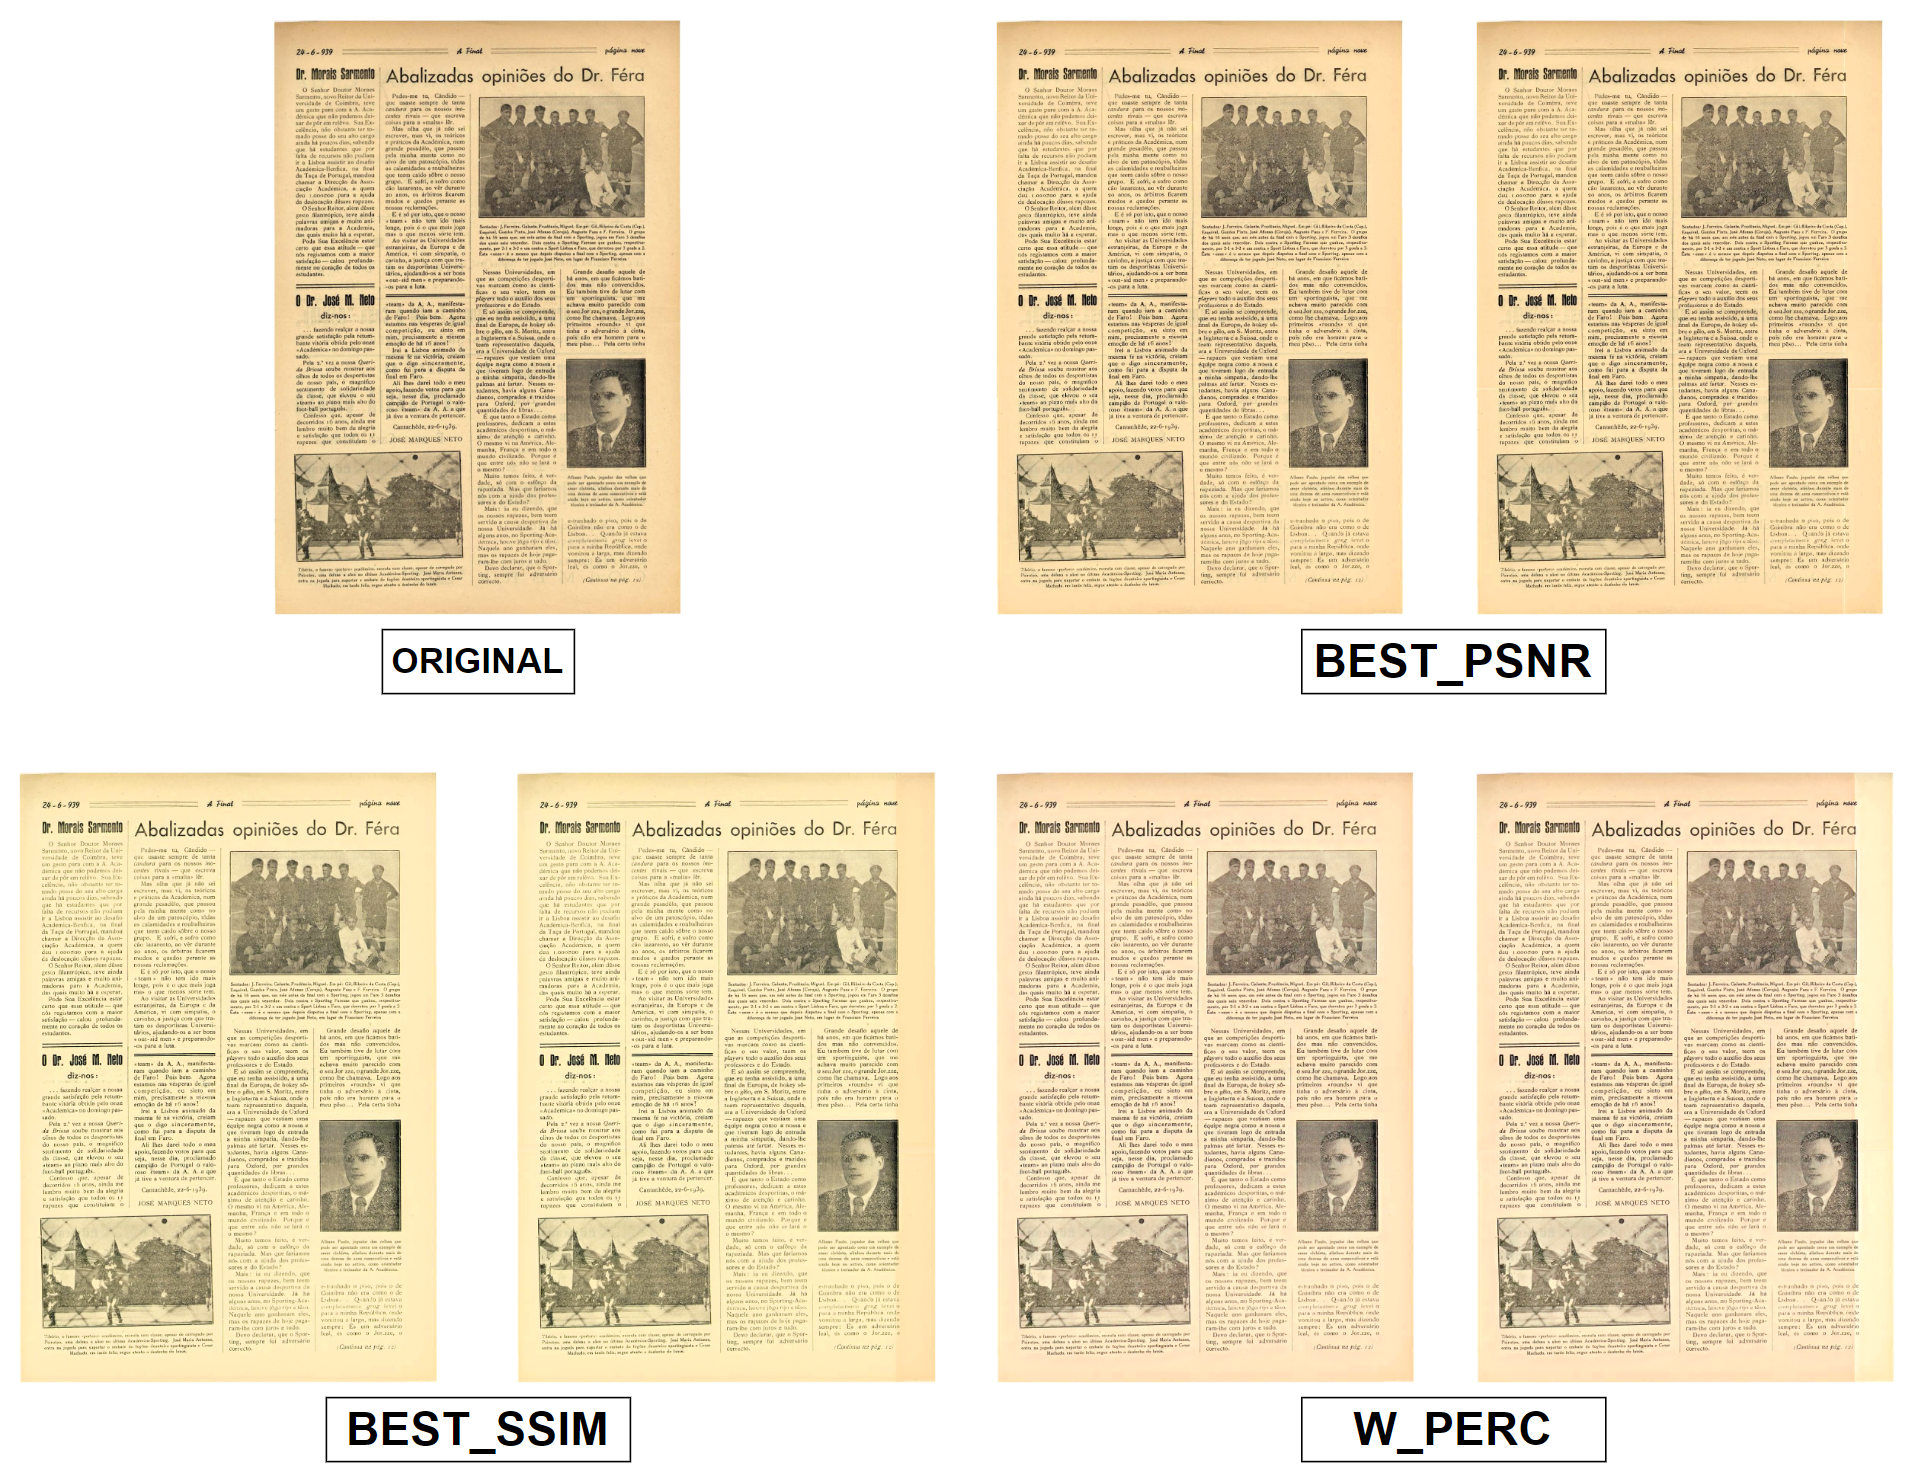
\includegraphics[width=0.7\textwidth]{images/ilustracoes/fix_illumination_example.png}
	\caption{Resultado de uso de diferentes modelos de correção de iluminação. Do lado esquerdo de cada modelo tem o resultado de uso sem divisão da imagem, e do lado direito o uso com divisão. Esta é uma imagem de resolução 1103x1612, já demonstrando para alguns modelos irregularidades no patch direito.}
	\label{fig:fix_illumination_example}
\end{figure}


\section{OCR}


Seguindo na pipeline, temos a a aplicação de OCR para extração do conteúdo textual de uma imagem. No caso de input do tipo OCR Tree - ou seu convertível -, este passo é ignorado, caso contrário é obrigatório.

% OCR de imagem

Ao longo da implementação e estudo dos resultados desta, foi utilizado \textbf{Tesseract} para a realização de OCR, devido a ser uma ferramenta open-source no topo do estado da arte.

O processo de OCR da pipeline pode ser dividido em blocos menores, sendo estes:

\begin{figure}[H]
	\centering
	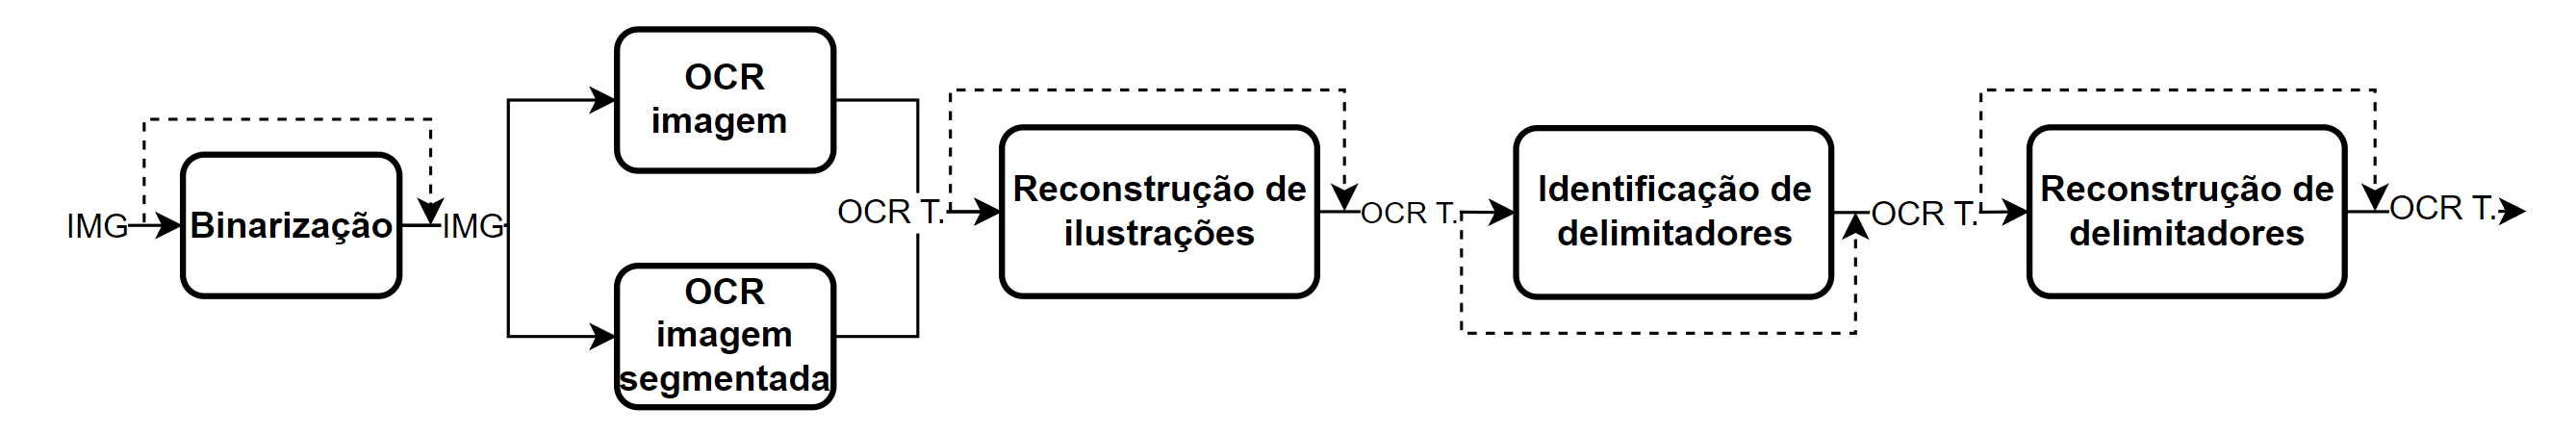
\includegraphics[width=1\textwidth]{images/diagramas/arquitetura_pipeline_ocr.png}
	\caption{Pipeline - secção OCR}
	\label{fig:arquitetura_pipeline_ocr}
\end{figure}


\highlight{Binarização}

%% binarizacao

A binarização de imagem é um processo que permite a realização de redução de ruído através da aplicação de tresholds, assim como a acentuação do texto de documentos. Este passo é também recomendado na documentação do Tesseract..

Este passo pode ser ignorado na pipeline, até pois o Tesseract internamente irá aplicar uma binarização própria.

A pipeline apresenta a opção de realizar binarização utilizando \textbf{Otsu} ou estilo \textbf{Fax}.



\highlight{OCR em imagem}

%%% imagem simples

A aplicação de OCR é realizada utilizando \textbf{Tesseract} podendo, através dos argumentos da pipeline, modificar a configuração deste, por exemplo: linguagem do texto a detetar; dpi da imagem; modo de segmentação.

Os resultados de OCR serão transformados numa OCR Tree.

\highlight{OCR em imagem segmentada}

%%% imagem segmentada

Em muitos casos, os documentos antigos apresentam variações do seu estado ao longo do documento. Por este motivo, a pipeline permite a habilidade de realizar um reconhecimento de texto aos diferentes segmentos da imagem, invés de numa única passagem. 

Para isto, podem ser passados os segmentos esperados na consola: 'header' , 'body' e 'footer'. Utilizando métodos de processamento de imagem do Toolkit, o documento será dividido nestes segmentos, particularmente o body será possivelmente ainda dividido em colunas, que serão separadamente binarizados (se intendido) e analisados com OCR.

Em seguida as diferentes OCR Tree resultantes serão unidas numa única.


\highlight{Reconstrução de delimitadores e imagens nos resultados}

%% incluir imagens e delimitadores identificados

Com a OCR Tree obtida, o último passo desta secção passa pela reconstrução de elementos não textuais do documento na OCR Tree. 

Estes são: ilustrações reconhecidas durante o pré-processamento; delimitadores identificados utilizando o Toolkit (se intendido).

Os elementos serão adicionados na OCR Tree, removendo blocos vazios que se situem dentro ou a intersetar com estes novos elementos.



\section{Pós-processamento de OCR}

% tratamento de resultados


Esta secção trata maioritariamente de manipulação da estrutura OCR Tree. A manipulação desta tem, naturalmente, consequências no texto reconhecido, e.x.: processos de eliminação de blocos vazios, estes são reconhecidos através do treshold de confiança definido, sendo que na realidade poderão conter texto.

Esta secção é também o segundo ponto de entrada da pipeline, sendo possível aceder diretamente a este através de um input do tipo Json ou HOCR, convertível para OCR Tree.


\begin{figure}[H]
	\centering
	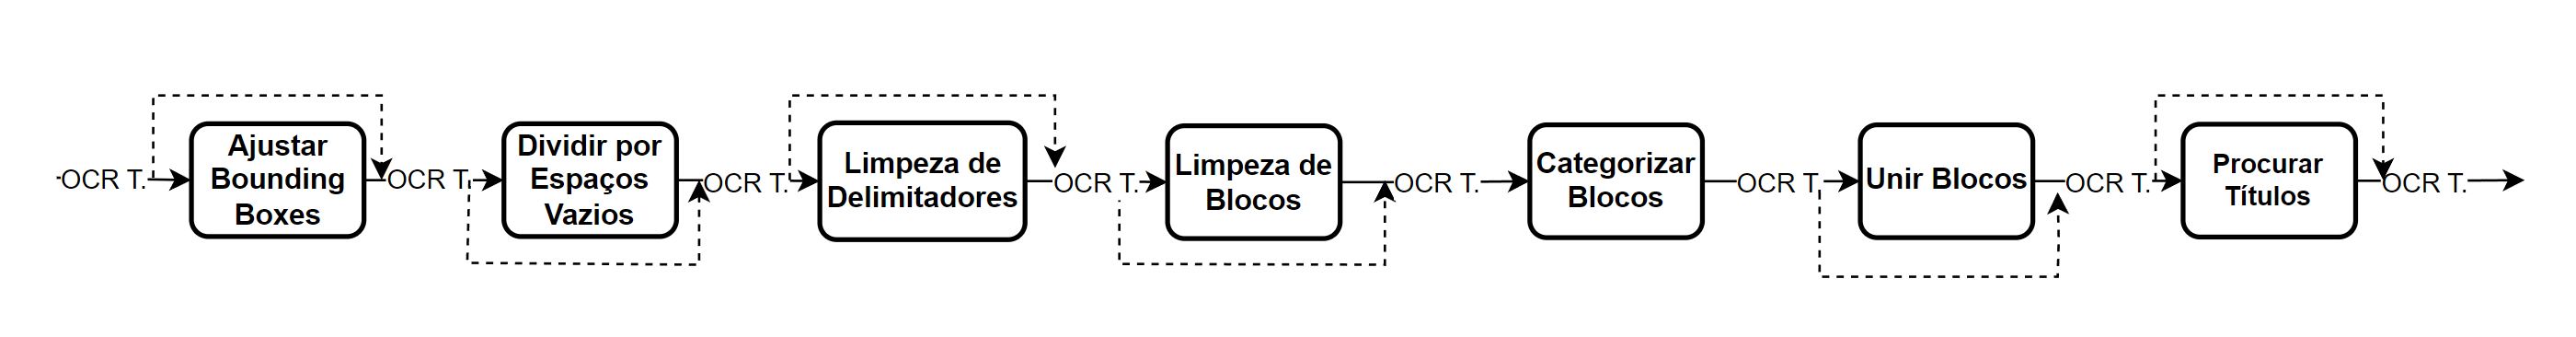
\includegraphics[width=1\textwidth]{images/diagramas/arquitetura_pipeline_posprocess.png}
	\caption{Pipeline - secção pós-processamento}
	\label{fig:arquitetura_pipeline_posprocess}
\end{figure}


%% clean OCR
\highlight{Remover blocos vazios}

Assumindo um valor de confiança de texto para ser vir de treshold, são removidos os blocos sem texto dos resultados. Estes são usualmente ruído que foi erradamente detetado como texto. 

São exceções imagens e delimitadores, que no caso do Tesseract, são detetados como blocos vazios. Dependendo da configuração da pipeline estes são detetados de diferentes formas, como já foi descrito.



\highlight{Ajustar Bounding Boxes}

O primeiro bloco de ação tem como objetivo reduzir a dimensão das bounding boxes dos blocos. Isto consegue-se através do valor dado para treshold de confiança de texto. Fazendo uso deste e do método 'text\_bound\_box\_fix', faz-se uma análise dos nodos de texto dentro dos blocos e, quando ignorados os de confiança abaixo da mínima, é possível reduzir a dimensão do bloco.

Esta ação é importante para diminuir possíveis interseções entre os blocos, normalmente causadas por deteções de ruído como texto. A redução destas interseções auxilia outras ações, como união de blocos ou cálculo da ordem de leitura.


\begin{figure}[H]
	\centering
	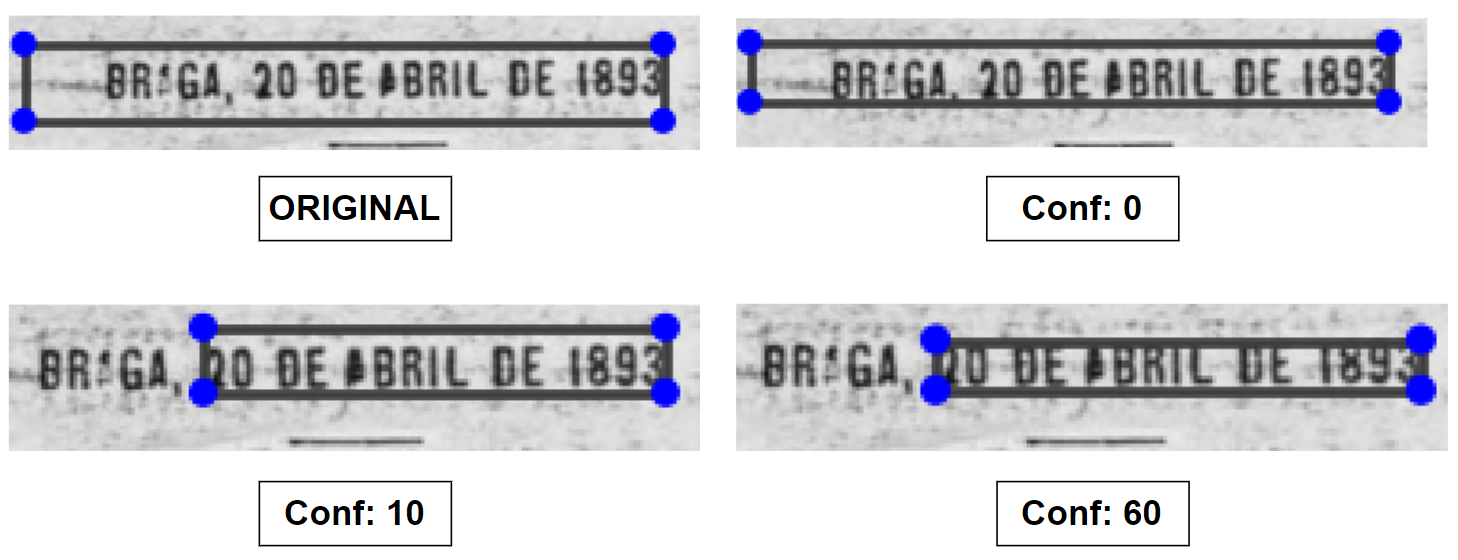
\includegraphics[width=0.7\textwidth]{images/ilustracoes/adjust_bounding_boxes_example.png}
	\caption{Resultado de passo de ajuste de bounding boxes utilizando diferentes valores de \textit{conf}.}
	\label{fig:adjust_bounding_boxes_example}
\end{figure}


\highlight{Dividir por espaços vazios}

A ação seguinte tem o intuito de dividir texto separado por um considerável espaço vazio em mais do que um bloco. Tal tem tendência a ocorrer na área de menção dos autores de artigos ou ilustrações.

Este bloco é conseguido usando o método 'split\_whitespaces'. Os parâmetros de confiança de texto e a razão entre o valor normal de espaço vazio e um válido de separação, são as principais influencias no desempenho deste passo.



\highlight{Limpeza de delimitadores}

Tanto no caso de delimitadores detetados através de métodos de análise de imagem, ou por heurísticas de dimensão dos blocos vazios, é expectável a presença de ruído, e.x.: delimitadores que foram detetados através do texto de título do jornal por este ser muito acentuado.

Deste modo, a limpeza destes é um passo recomendado. Esta consegue-se através de um método criado para este propósito da pipeline: 'delimiters\_fix'. Este método analisa os delimitadores e, validadas certas condições, aplica limpezas, ex.: delimitador inserido completamente dentro de texto -> remove delimitador; delimitador a intersetar com texto -> ajusta bounding box do delimitador.


\highlight{Limpeza de blocos}

Segue-se o passo de limpeza geral de blocos, tratando casos de interseções, blocos vazios e blocos inseridos em outros. Para isto é usado o método 'block\_bound\_box\_fix'.


\begin{figure}[H]
	\centering
	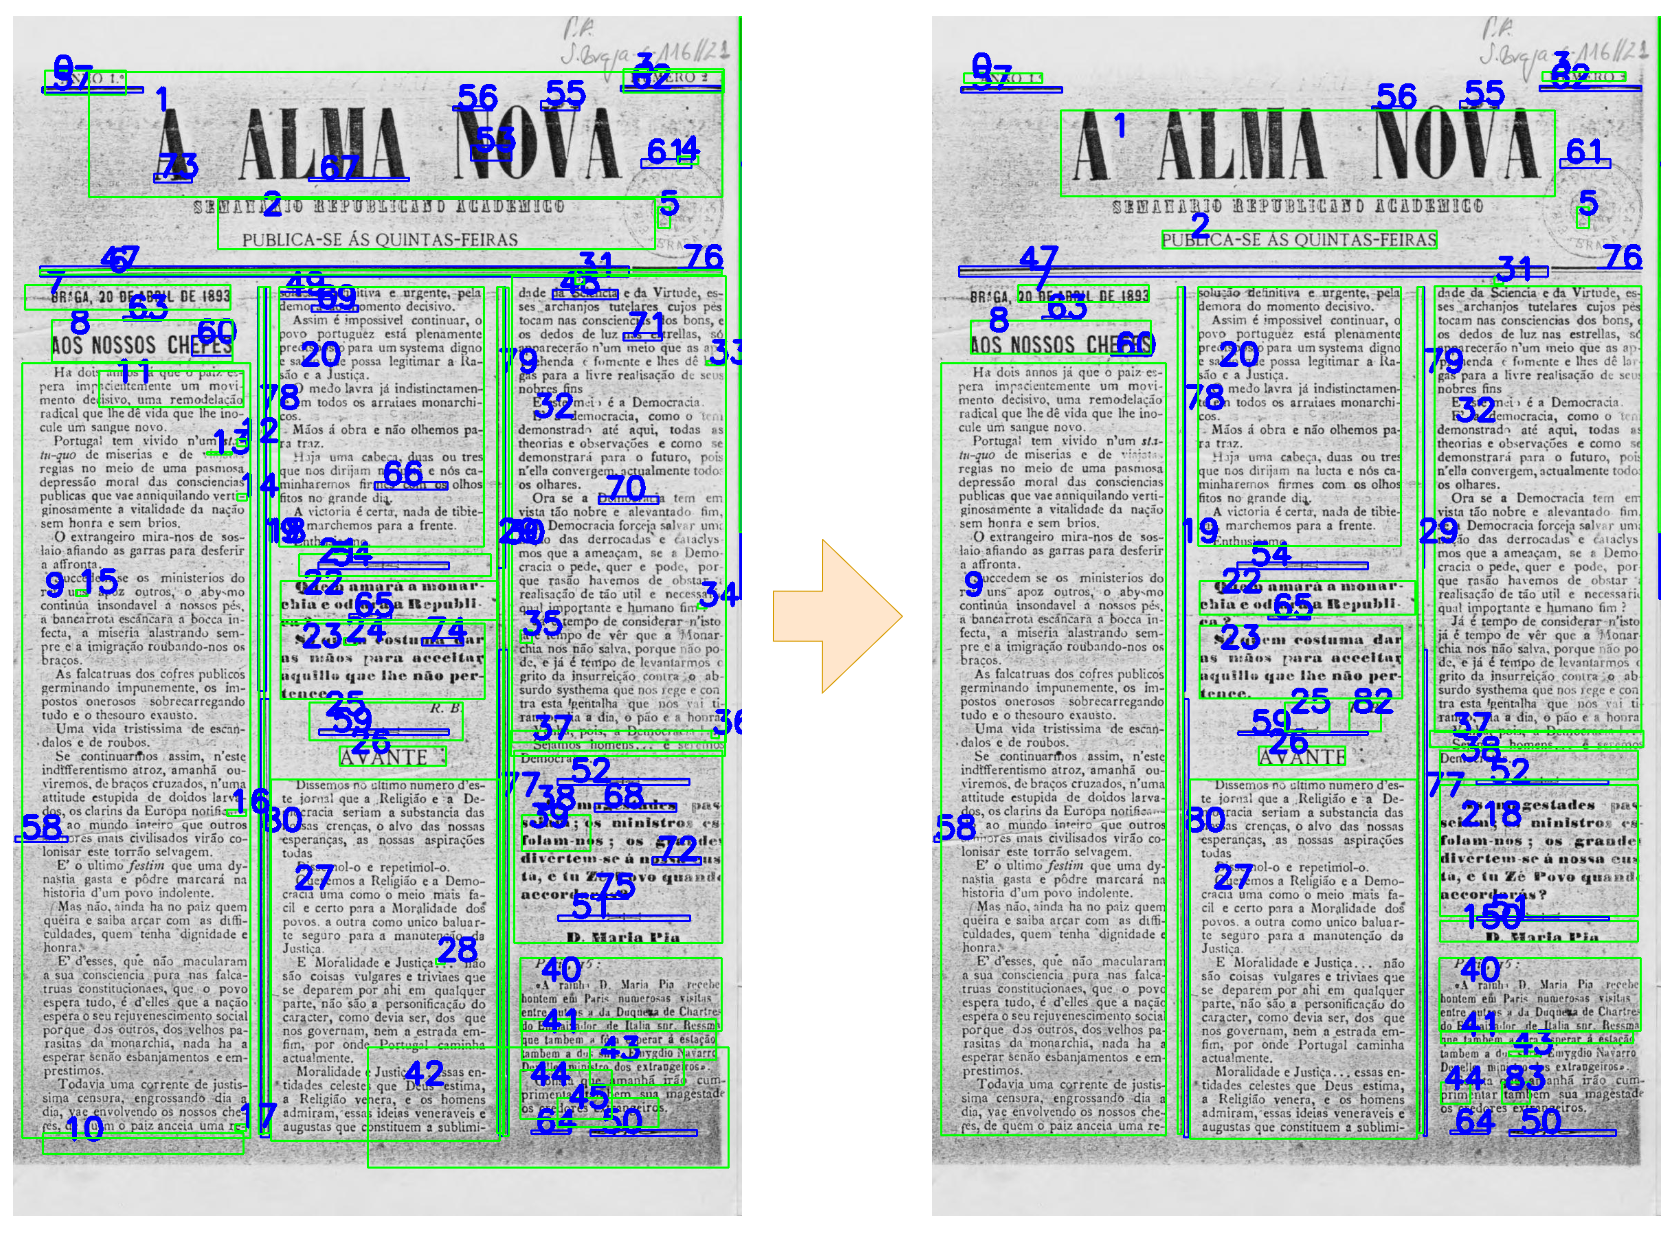
\includegraphics[width=0.7\textwidth]{images/ilustracoes/pipeline_clean_ocr_example.png}
	\caption{Resultado de aplicação dos passos de limpeza (passos até agora listados) dos resultados OCR.}
	\label{fig:pipeline_clean_ocr_example}
\end{figure}


%% categorizacao OCR
\highlight{Categorização de blocos}

O passo de categorização de blocos é essencial para as ações posteriores de união de blocos, procura por títulos e cálculos de atração entre blocos. Não sendo uma ação impactante da OCR Tree, apenas atualizando o atributo 'type'. Este é um passo obrigatória na pipeline.

\begin{figure}[H]
	\centering
	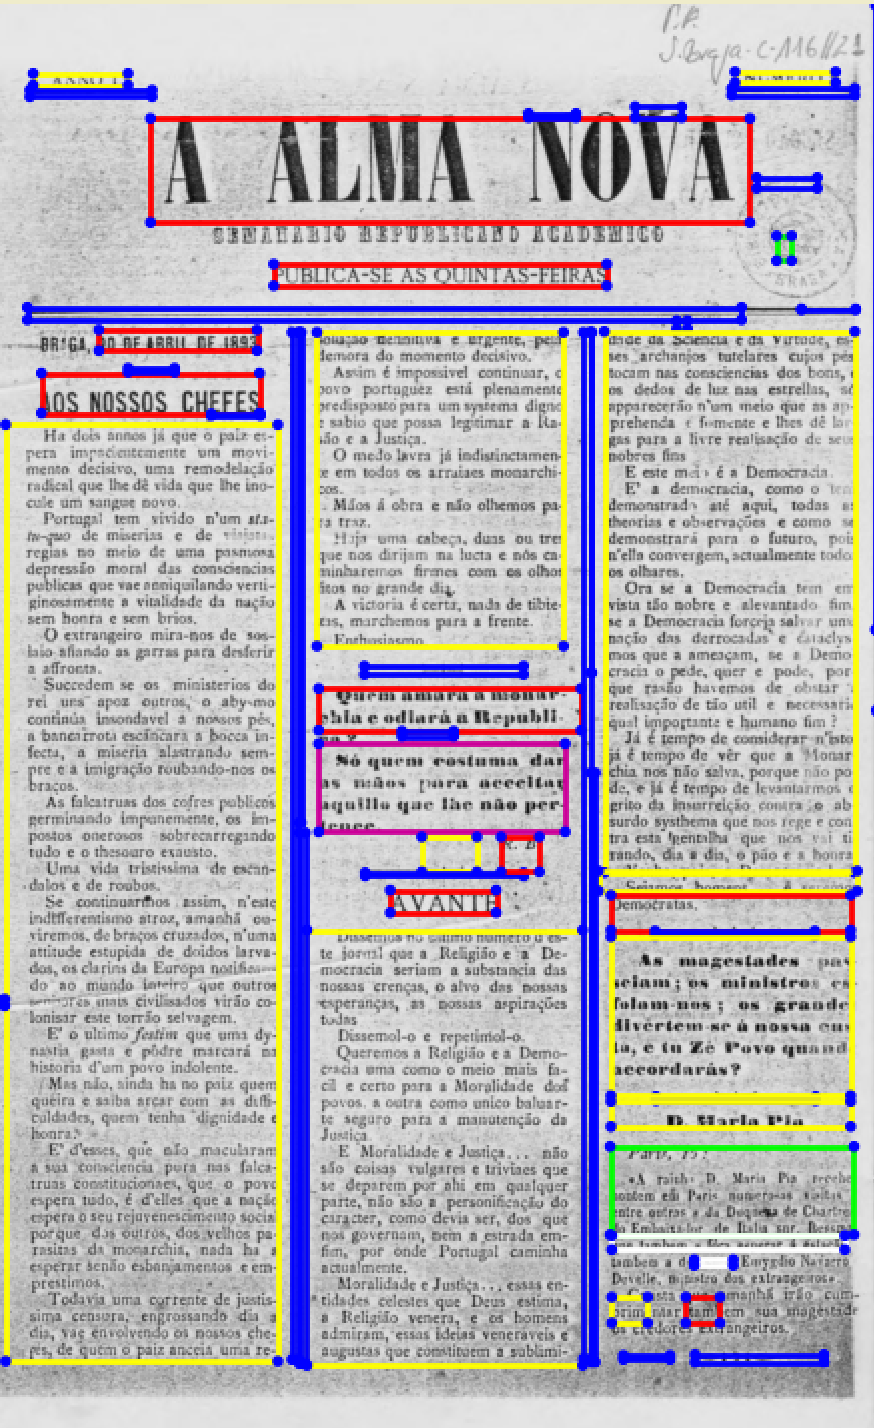
\includegraphics[width=0.3\textwidth]{images/ilustracoes/pipeline_categorize_ocr_example.png}
	\caption{Resultado de aplicação do passo de categorização de blocos.}
	\label{fig:pipeline_categorize_ocr_example}
\end{figure}



%% Uniao OCR
\highlight{União de blocos}

A união de blocos auxilia o passo de cálculo da ordem de leitura, e realiza uma simplificação da OCR Tree. O objetivo é a redução da quantidade de blocos existente ao unir aqueles que são do mesmo tipo e aceitam determinadas condições geométricas.

A união de blocos pode realçar posição relativa entre estes e outros que anteriormente não eram expressas, potencializando o cálculo da atração entre blocos.



%% Find titles
\highlight{Procura por títulos}


O bloco de procura por títulos pretende corrigir casos em que a segmentação em blocos do motor OCR uniu texto com potencial de título (de artigo sendo esse o foco do projeto) do texto seguinte.

Tal permitirá em passos seguintes, de isolamento dos artigos, a identificação de mais artigos do que na ausência deste passo, dado que os artigos são distinguidos pela deteção de títulos.

No caso de serem detetados novos títulos, o método 'find\_text\_titles' irá dividir o bloco de texto, gerando o novo bloco título e 1 a 2 (dependendo da posição relativa do título) blocos texto.

\begin{figure}[H]
	\centering
	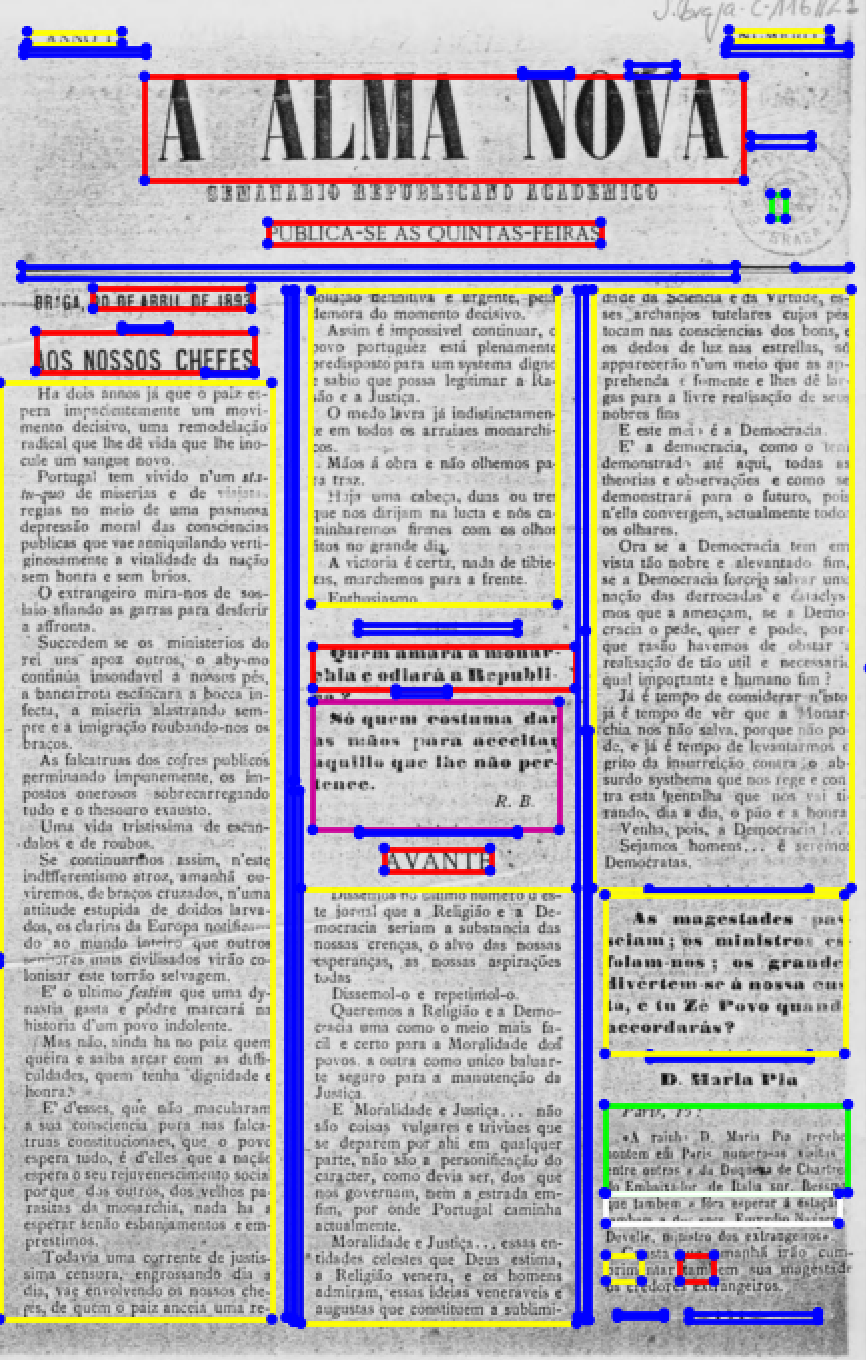
\includegraphics[width=0.3\textwidth]{images/ilustracoes/pipeline_final_example.png}
	\caption{Resultado final de pós processamento dos resultados de OCR.}
	\label{fig:pipeline_final_example}
\end{figure}



\section{Geração de output}

A última secção da pipeline passa pela geração do output final em formato textual. 

Nesta, a pipeline da opção de escolher: a geração dedicada a jornais, onde a flag 'extract\_articles' está ativa e portanto os artigos serão isolados para o output final; ou output simples. Em ambos os casos é ainda possível aplicar o bloco de cálculo da ordem de leitura e escolher o formato do output textual.

Os formatos para output final disponíveis são: texto simples; markdown.

\begin{figure}[H]
	\centering
	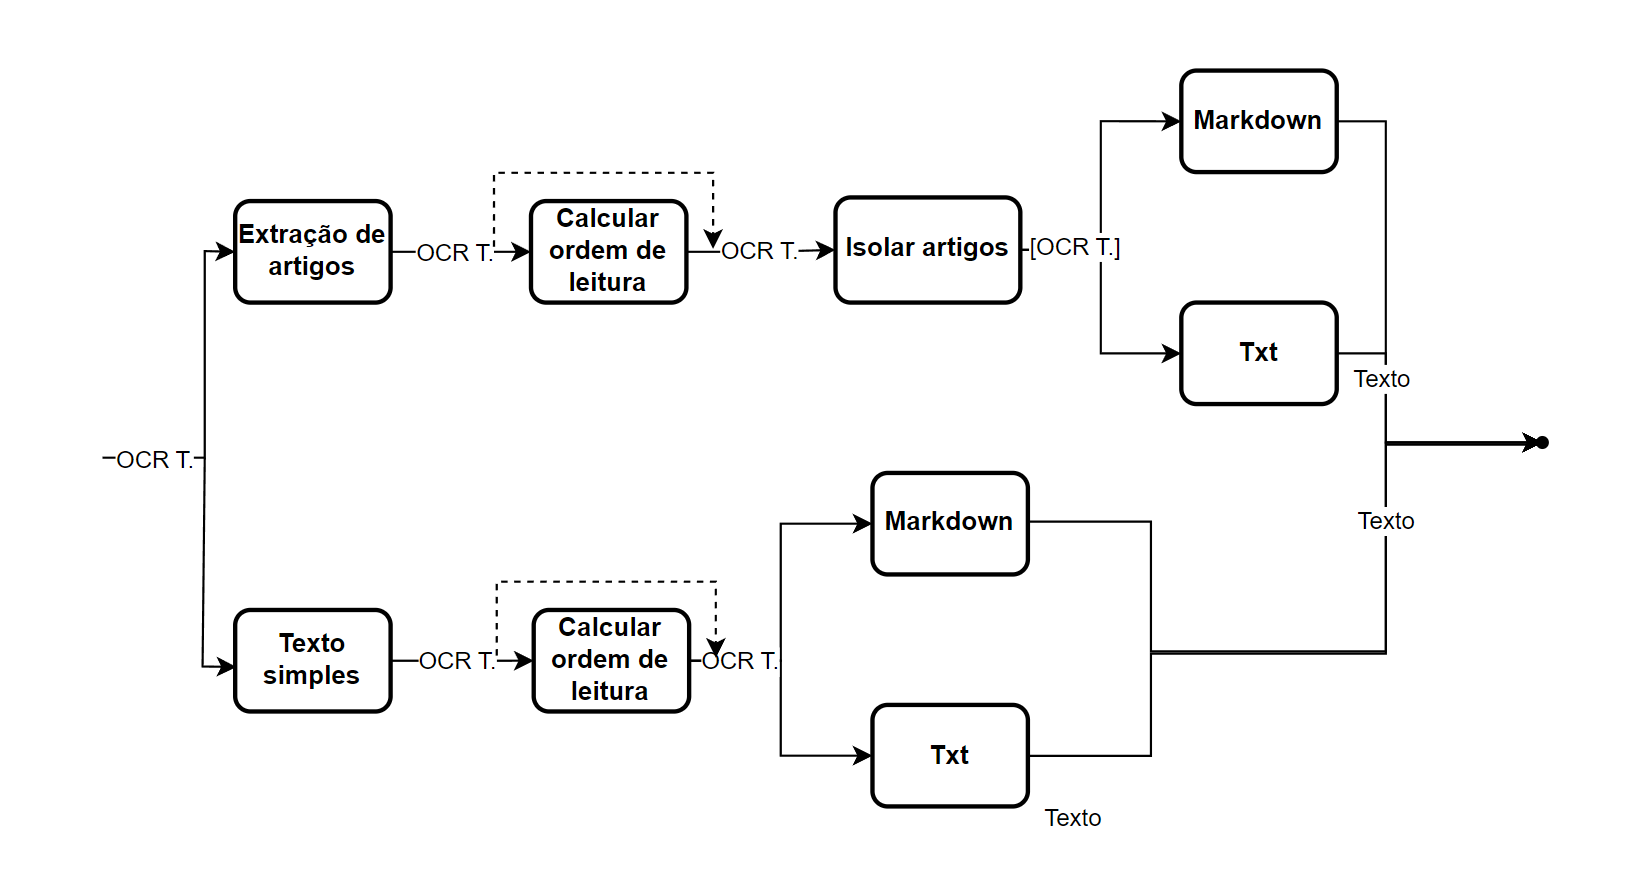
\includegraphics[width=0.8\textwidth]{images/diagramas/arquitetura_pipeline_output.png}
	\caption{Pipeline - secção output}
	\label{fig:arquitetura_pipeline_output}
\end{figure}

% criacao de output
%% output para jornal
%%% calculo da ordem de leitura
%%% output para text
%%% output para markdown
%% output simples
%%% output text


\highlight{Cálculo da ordem de leitura}

O bloco de cálculo da ordem de leitura pretende, através do cálculo de atração entre blocos - que dependem das características dos blocos assim como posições relativas - do corpo do documento, e de uma ordenação topológica pesada, gerar uma ordenação mais próxima da intendida do que originalmente decidida pelo motor OCR. Como explicitado anteriormente, os algoritmos desenhados têm um foco na ordenação de jornais.


\begin{figure}[H]
	\centering
	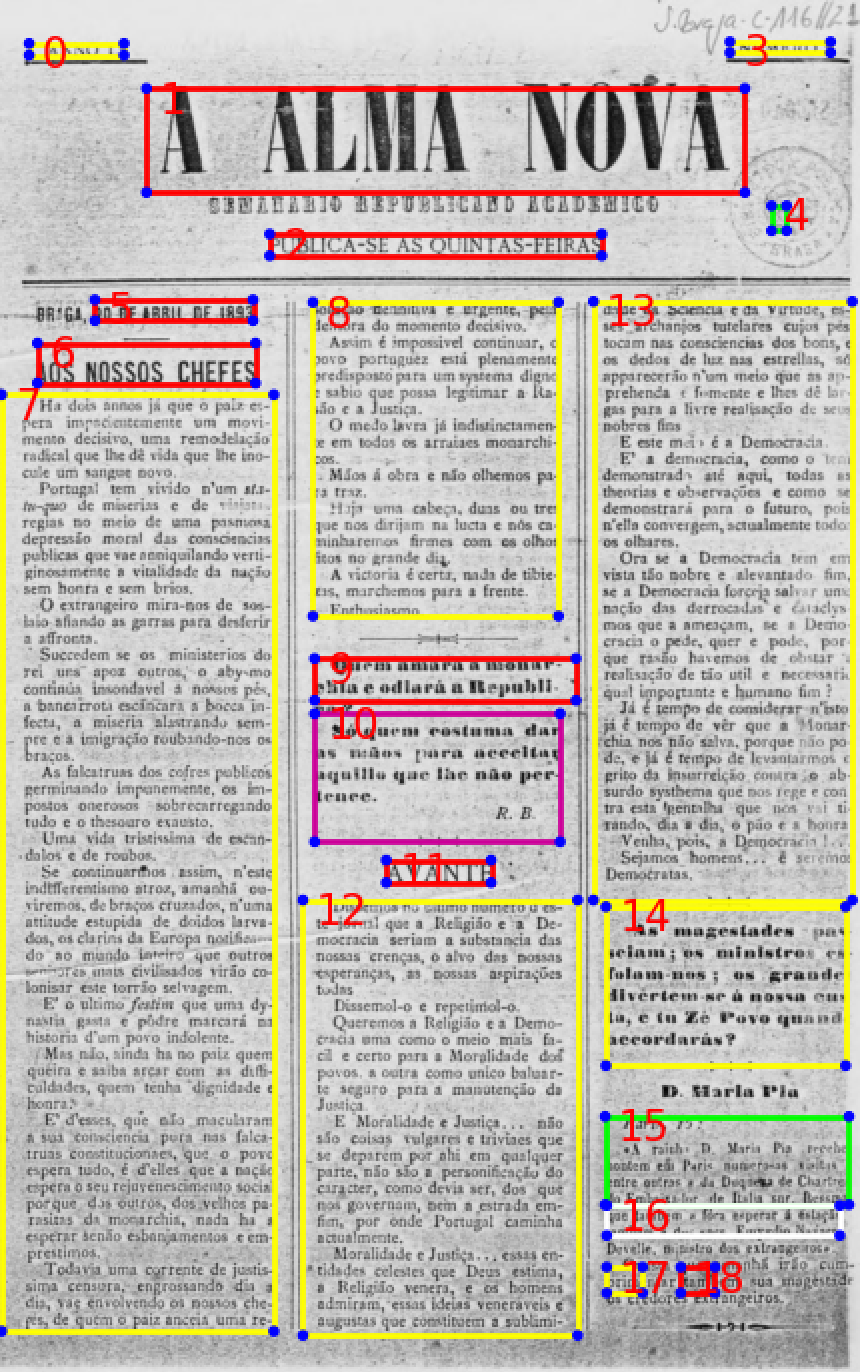
\includegraphics[width=0.3\textwidth]{images/ilustracoes/pipeline_calculate_reading_order_example.png}
	\caption{Resultado de cálculo da ordem de leitura.}
	\label{fig:pipeline_calculate_reading_order_example}
\end{figure}

\highlight{Isolamento de artigos}


O passo de isolamento de artigos procura, dentro da lista de blocos ordenados, segmentá-los em diferentes artigos. Os artigos são caracterizados por serem iniciados por um título e possuírem texto além deste.

O resultado final será uma lista de listas OCR Tree do nível bloco, i.e. uma lista de artigos.

\begin{figure}[H]
	\centering
	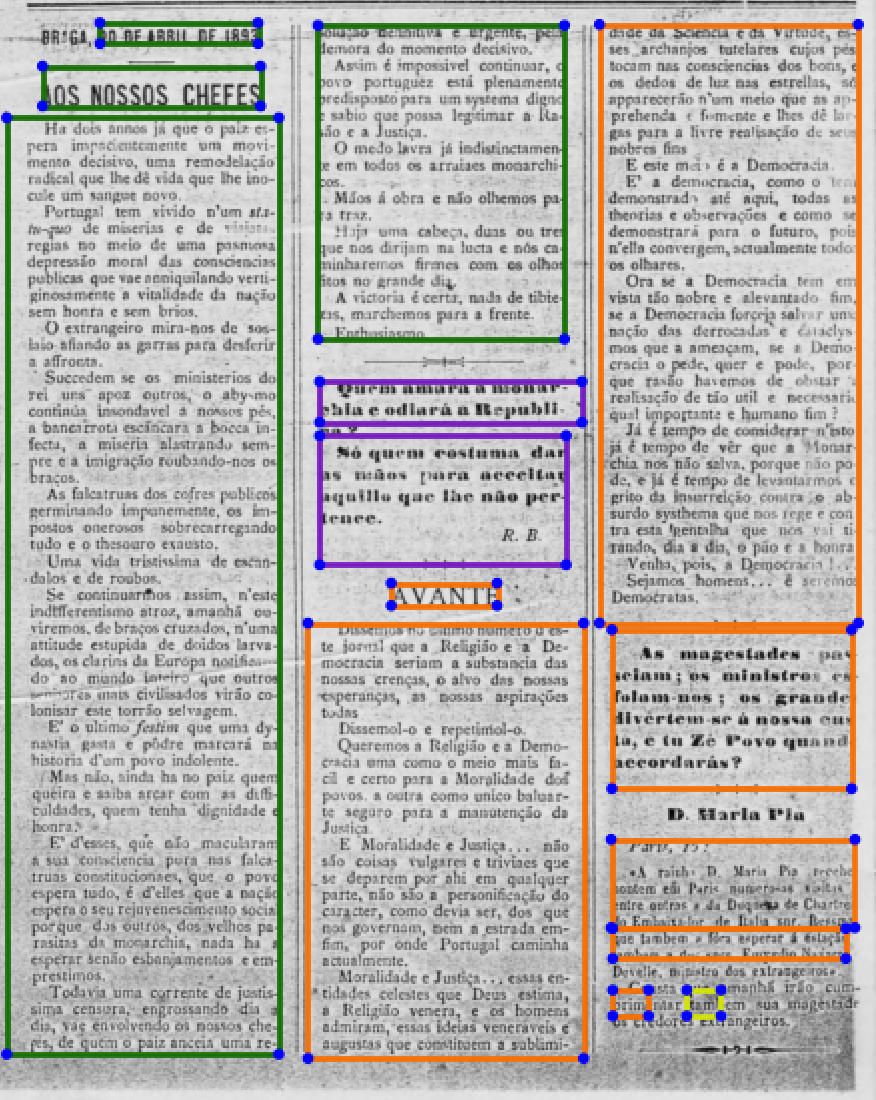
\includegraphics[width=0.3\textwidth]{images/ilustracoes/pipeline_isolate_articles_example.png}
	\caption{Resultado de isolamento de artigos.}
	\label{fig:pipeline_isolate_articles_example}
\end{figure}



\highlight{Output final}

O output final será sempre em formato textual. Este pode ser do tipo markdown ou texto simples, e do tipo documento jornal ou outro. 

No caso de documento jornal, o algoritmo irá utilizar os artigos isolados e, por ordem, transcrevê-los no output. Para outro tipo, apenas transcreve os blocos da forma como foram ordenados.

Em particular para o formato markdown, tendo em conta a possibilidade de incluir imagens neste formato, blocos do tipo imagem identificados durante a pipeline, serão incluídos no output final na posição indicada pela ordem final de blocos/artigos.



\section{Validação de resultados}

O comando que aciona a pipeline apresenta ainda uma aplicação alternativa. Esta outra aplicação é dedicada à verificação/validação dos resultados da utilização da pipeline e, consequentemente, calibrar a mesma.

Esta utilização, ao contrário da pipeline, não é de independente do utilizador, necessitando que este provisione recursos extra além da imagem de input inicial. Estes recursos extra são respetivos a resultados esperados do output: ground truth total; ground truth parcial; ficheiro de resultados esperadas. Destes, pelo menos uma das ground truth deve ser fornecida. Além disso, pelo menos uma pipeline tem de ser fornecida para serem analisados os seus resultados no input.

O caso de uso esperado é a de, para uma coleção de um dado jornal, em que as diferentes edições têm características semelhantes, o utilizador forneça para uma destas estes recursos para comparação, assim como uma lista compreensiva de diferentes pipelines com diferentes configurações que serão comparadas e, entre estas, serão escolhidas as opções que melhores resultados obtiveram.

Os métodos utilizados nesta funcionalidade são, na generalidade, dedicados à mesma, não tendo sido implementados com a mesma filosofia de independência do toolkit.

\highlight{Ground truth total}

A ground truth total trata-se de uma transcrição completa do texto do documento.


\highlight{Ground truth parcial}

A ground truth parcial trata-se de uma transcrição de apenas alguns trechos do documento, que devem estar ordenados corretamente, ex.: uma frase de cada uma dos artigos do jornal.

\highlight{Ficheiro de resultados esperados}

O ficheiro de resultados contém informação além do output textual final. Este pode conter: o número de artigos que o output final deve ter; número de ilustrações que o documento contém; número de colunas do jornal.


\highlight{Comparação dos resultados e calibração da pipeline}

Dada um conjunto de pipelines para serem comparadas, para cada uma seguirá o seguinte processo:

\textbf{Aplicação da pipeline no input}, guardando os seus outputs numa pasta própria.

\textbf{Apuramento dos resultados} da pipeline, nomeadamente: 

\begin{itemize}\setlength\itemsep{-0.3em}
	\item nível médio da confiança do texto
	\item número de palavras
	\item similaridade de cosseno entre o texto e a ground truth total
	\item número de linhas iguais entre ground truth parcial e o texto
	\item número de linhas iguais entre ground truth parcial e o texto na ordem certa
	\item número de colunas detetadas
	\item número de ilustrações detetadas
	\item número de artigos detetados
\end{itemize}


\textbf{Atribuição de uma classificação} numérica a cada secção da pipeline ao comparar os resultados obtidos com os recursos dos resultados esperados. As secções classificadas são o pré processamento e o pós processamento.

\textbf{Calibração da pipeline} ao comparar os diferentes classificações das pipelines e, escolhendo para cada secção as configurações da pipeline (respetivas à dada secção) que nela teve melhor classificação.

É também possível apenas realizar a classificação de uma pipeline única.










